%!TEX TS-program = xelatex
%!TEX encoding = UTF-8 Unicode

\documentclass[11pt,tikz,border=1]{standalone}
\usetikzlibrary{positioning}

\begin{document}
  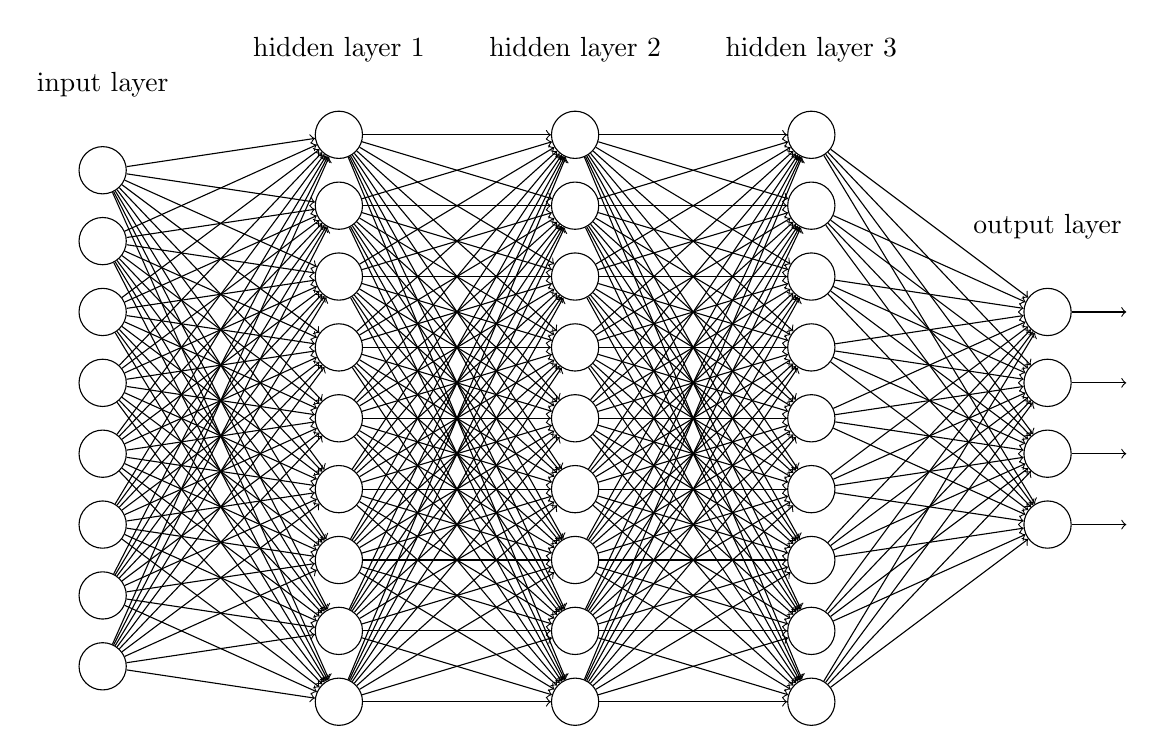
\begin{tikzpicture}[
    neuron/.style={circle,draw,inner sep=0pt,minimum size=6mm}
    ]

    \foreach \y in {0,...,7}
      \node(i\y) [neuron] at (0,\y * 0.9 + 0.45) {};

    \foreach \y in {0,...,8}
      \node(h1\y) [neuron] at (3,\y * 0.9) {};

    \foreach \y in {0,...,8}
      \node(h2\y) [neuron] at (6,\y * 0.9) {};

    \foreach \y in {0,...,8}
      \node(h3\y) [neuron] at (9,\y * 0.9) {};

    \foreach \y in {0,...,3}
      \node(o\y) [neuron] at (12,\y * 0.9 + 2.25) {};

    \node [above=0.5 of i7] {input layer};
    \node [above=0.5 of h18] {hidden layer 1};
    \node [above=0.5 of h28] {hidden layer 2};
    \node [above=0.5 of h38] {hidden layer 3};
    \node [above=0.5 of o3] {output layer};

    \foreach \x in {0,...,7}
      \foreach \y in {0,...,8}
        \draw[->] (i\x) to (h1\y);

    \foreach \x in {0,...,8}
      \foreach \y in {0,...,8}
        \draw[->] (h1\x) to (h2\y);

    \foreach \x in {0,...,8}
      \foreach \y in {0,...,8}
        \draw[->] (h2\x) to (h3\y);

    \foreach \x in {0,...,8}
      \foreach \y in {0,...,3}
        \draw[->] (h3\x) to (o\y);

    \foreach \y in {0,...,3}
      \draw[->] (o\y) -- ++(1,0);

  \end{tikzpicture} 
\end{document}
